\documentclass{article}

% NeurIPS 2025 style
\usepackage[final]{neurips_2024}

% Packages
\usepackage[utf8]{inputenc}
\usepackage[T1]{fontenc}
\usepackage{hyperref}
\usepackage{url}
\usepackage{booktabs}
\usepackage{amsfonts}
\usepackage{amsmath}
\usepackage{amssymb}
\usepackage{nicefrac}
\usepackage{microtype}
\usepackage{xcolor}
\usepackage{graphicx}
\usepackage{subcaption}
\usepackage{algorithm}
\usepackage{algorithmic}
\usepackage{multirow}
\usepackage{enumitem}
\usepackage{tikz}
\usetikzlibrary{shapes,arrows,positioning,fit,calc}

% Custom commands
\newcommand{\heron}{\textsc{Heron}}
\newcommand{\ie}{\textit{i.e.}}
\newcommand{\eg}{\textit{e.g.}}
\newcommand{\etal}{\textit{et al.}}
\newcommand{\todo}[1]{\textcolor{red}{[TODO: #1]}}
\newcommand{\placeholder}[1]{\textcolor{blue}{[PLACEHOLDER: #1]}}
\newcommand{\exampleval}[1]{\textcolor{teal}{#1}\textsuperscript{\textcolor{teal}{$\dagger$}}} % preliminary value (to be replaced by final benchmark results)
\newcommand{\cmark}{\checkmark}
\newcommand{\xmark}{$\times$}

\title{\heron{}: Event-Driven, Agent-Centric Simulation for Asynchronous MARL Benchmarks}

\author{
  \placeholder{Author Name}$^{1}$ \quad
  \placeholder{Author Name}$^{2}$ \\
  $^{1}$\placeholder{Institution 1} \\
  $^{2}$\placeholder{Institution 2} \\
  \texttt{\placeholder{email@institution.edu}}
}

\begin{document}

\maketitle

\begin{abstract}
Multi-agent reinforcement learning (MARL) benchmarks are largely built around an \emph{environment-centric} and \emph{synchronous} execution model: a single environment loop advances a global clock, broadcasts observations, and collects actions from all agents. This ``global clock'' abstraction is convenient for games and turn-based settings, but it obscures two realities that dominate real cyber-physical systems (CPS): (i) \emph{agents operate at heterogeneous decision rates} with nontrivial observation/action latencies, and (ii) \emph{information is partitioned} by organizational and privacy boundaries rather than globally broadcast. These mismatches make it difficult to benchmark robustness to timing uncertainty, study privacy-preserving coordination, or validate decentralized algorithms before deployment.

We introduce \heron{}, a simulation and benchmark framework that makes \textbf{time}, \textbf{information access}, and \textbf{interaction protocols} first-class experimental variables. \heron{}'s core idea is an \textbf{event-driven, agent-centric} execution model: agents are autonomous entities that act when scheduled, while the environment serves as a physics oracle and event manager. Building on this foundation, \heron{} provides: (1) an \textbf{event-driven engine} that supports heterogeneous decision cycles and configurable observation/action/message delays; (2) \textbf{ProxyAgents} and visibility-labeled \textbf{FeatureProviders} to enforce strict data isolation and role-based partial observability (\texttt{public}, \texttt{owner}, \texttt{upper\_level}, \texttt{system}); and (3) a modular \textbf{protocol system} that decouples coordination semantics from actuation, enabling controlled comparisons of centralized, hierarchical, and peer-to-peer interaction patterns.

To demonstrate benchmark readiness, we instantiate \heron{} for multi-microgrid coordination using PandaPower-based AC power flow and provide standard IEEE/CIGRE feeders, reference scenarios, and classical baselines. \heron{} is released open-source to support reproducible research on asynchronous, information-constrained multi-agent coordination.
\end{abstract}

%==============================================================================
\section{Introduction}
\label{sec:intro}
%==============================================================================

MARL has achieved strong results in game-like benchmarks \cite{samvelyan2019starcraft, vinyals2019grandmaster}, but real-world deployment in networked systems remains brittle. A core reason is a \textbf{simulation mismatch}: many benchmarks encode assumptions that collapse in cyber-physical systems (CPS) such as smart grids, traffic networks, and robot fleets.

\paragraph{First principle: what the benchmark should control.}
In real distributed control, three design dimensions are inseparable:
\begin{itemize}[nosep]
    \item \textbf{Time}: agents act at different rates (milliseconds to hours), and observations/actions traverse networks with latency.
    \item \textbf{Information}: observations are filtered by organizational roles, privacy policies, and bandwidth constraints.
    \item \textbf{Interaction}: coordination depends on explicit protocols (prices, setpoints, bids, consensus), not implicit global state broadcasts.
\end{itemize}

However, most MARL benchmarks present these dimensions as fixed implementation details. The prevalent paradigm is an \emph{environment-centric global step}: the environment exposes a \texttt{step()} API, advances time in lockstep, and returns observations that are often derived from a globally accessible simulator state.

\paragraph{Why the global clock breaks in CPS.}
Consider a distribution grid with many distributed energy resources (DERs). Field devices act on fast inverter loops, microgrid controllers coordinate on slower horizons, and supervisory layers update even more slowly. Communication (SCADA/industrial networks) introduces latency; commercial and security constraints prevent full-state sharing between stakeholders. Similar constraints arise in traffic control (heterogeneous signal timing and sensor delays) and robotics (distributed robots with bandwidth-limited coordination).

\paragraph{Key idea.}
This paper proposes a shift from environment-centric stepping to \textbf{event-driven, agent-centric simulation}. Instead of forcing all agents to synchronously observe and act, \heron{} models each agent as an independent entity with its own decision schedule. A discrete-event engine advances the simulation by processing \emph{events} (agent decisions, message deliveries, physics updates), making timing uncertainty, communication latency, and information boundaries explicit and configurable.

\paragraph{Contributions.}
\heron{} is a benchmark framework whose contributions align around this single theme---\emph{making time and information structure explicit in multi-agent simulation}:
\begin{enumerate}[leftmargin=*, itemsep=2pt]
    \item \textbf{Event-driven, agent-centric execution model} (\S\ref{sec:edac}): a discrete-event simulation substrate that supports heterogeneous decision cycles and stochastic latency for observation, action, and communication.
    \item \textbf{Physical--logical decoupling via ProxyAgents} (\S\ref{sec:proxy}): a managed mediation layer that enforces strict separation between an agent's private state and the environment's global state, enabling principled partial observability and privacy constraints.
    \item \textbf{Composable observability via FeatureProviders} (\S\ref{sec:observability}): modular, visibility-labeled feature blocks that enable systematic information ablations and controlled observability mismatches.
    \item \textbf{Protocol system for coordination topologies} (\S\ref{sec:protocols}): a modular interface to swap centralized, hierarchical, and peer-to-peer coordination schemes without rewriting environment physics.
    \item \textbf{Benchmark instantiation in power systems} (\S\ref{sec:power}): a benchmark-ready microgrid coordination suite with standard feeders, scenarios, and baselines to demonstrate how \heron{} is used in a real CPS setting.
\end{enumerate}

%==============================================================================
\section{Related Work}
\label{sec:related}
%==============================================================================

\textbf{Multi-agent benchmarks and environment APIs.}
MPE \cite{mordatch2018emergence} and SMAC \cite{samvelyan2019starcraft} popularized standardized MARL evaluation, but inherit synchronous time stepping and typically expose observations derived from a globally updated simulator state. PettingZoo \cite{terry2021pettingzoo} provides an important API standardization effort, especially for agent-environment cycling in games, but its default stepping abstractions do not model heterogeneous decision rates and network-induced latency as first-class benchmark variables.

\textbf{Distributed RL systems.}
RLlib focuses on scalable, composable abstractions for distributed RL training, separating algorithm logic from execution strategy. \heron{} is complementary: we focus on the \emph{environment and simulation side} and on representing timing and information constraints that shape what ``distributed execution'' means in CPS.

\textbf{Communication and hierarchy in MARL.}
Learned communication \cite{foerster2016learning, das2019tarmac} and hierarchical control \cite{vezhnevets2017feudal} study coordination under partial information. Surveys emphasize that communication topology, bandwidth, and latency are central drivers of performance (\todo{add citation to MARL communication survey}). \heron{} provides a simulation substrate where these assumptions can be varied systematically via visibility-labeled features, explicit message channels, and event-driven scheduling.

\textbf{Energy-domain RL benchmarks.}
Grid2Op \cite{donnot2020introducing} and gym-anm \cite{henry2021gym} provide realistic power-system simulators but are primarily single-agent. CityLearn \cite{vazquez2019citylearn} and PowerGridworld \cite{biagioni2022powergridworld} support multi-agent energy settings, but observability is typically monolithic (full vs. local), and realistic timing/latency is not exposed as a benchmark dimension. \heron{} targets the missing intersection: multi-agent CPS benchmarks with explicit information hierarchies and event-driven timing.

%==============================================================================
\section{From Global-Clock Stepping to Event-Driven Agent-Centric Simulation}
\label{sec:edac}
%==============================================================================

This section introduces the conceptual model that unifies \heron{}'s design.

\subsection{The Global-Clock Assumption}
Many MARL environments can be summarized as a synchronous loop:
\begin{equation}
    \text{observe } \{o^i_t\}_{i\in\mathcal{A}} \;\rightarrow\; \text{act } \{a^i_t\}_{i\in\mathcal{A}} \;\rightarrow\; \text{transition } s_{t+1}=T(s_t,\{a^i_t\})
\end{equation}
This abstraction implicitly assumes: (i) all agents share the same decision time $t$, (ii) observations are delivered without delay, and (iii) actions take effect synchronously. In CPS, none of these are guaranteed.

\subsection{Event-Driven Agent-Centric Execution}
\heron{} models a multi-agent system as a discrete-event process.

\paragraph{State.}
At simulation time $\tau$, the system consists of a \emph{physical state} $x(\tau)$ (maintained by the environment/physics backend), and \emph{agent-local states} $\{h_i(\tau)\}$ (private memory, local estimates, buffers).

\paragraph{Events.}
An event is a tuple $e=(\tau,\,\texttt{type},\,\texttt{payload})$ stored in a priority queue ordered by time. \heron{} uses three families of events:
\begin{itemize}[nosep]
    \item \textbf{Decision events}: deliver an observation to agent $i$, triggering a policy evaluation and scheduling a future action.
    \item \textbf{Delivery events}: deliver a message to an agent with explicit latency (including observation and protocol messages).
    \item \textbf{Physics events}: apply queued actions to the backend and run a physics update (\eg AC power flow).
\end{itemize}

\paragraph{Scheduling.}
Each agent $i$ has a decision interval $\Delta_i$ and delay models $d^{\text{obs}}_i$, $d^{\text{act}}_i$; communication channels have message delay $d^{\text{msg}}$. These can be deterministic or stochastic. Synchronous stepping is recovered as the special case where all $\Delta_i$ are equal and all delays are zero.

\begin{algorithm}[t]
\caption{Discrete-event simulation loop (distributed mode)}
\label{alg:event-loop}
\begin{algorithmic}[1]
\REQUIRE Priority queue $Q$ of timestamped events
\WHILE{not terminal}
    \STATE $(\tau,\texttt{type},\texttt{payload}) \gets \texttt{pop\_min}(Q)$
    \STATE advance simulation time to $\tau$
    \IF{$\texttt{type} = \texttt{DELIVER}$}
        \STATE deliver message to target agent (subject to visibility filtering)
    \ELSIF{$\texttt{type} = \texttt{DECIDE}$}
        \STATE compute agent observation $o_i = \texttt{ProxyFilter}(x(\tau), i)$
        \STATE agent returns action proposal $a_i \sim \pi_i(o_i, h_i)$
        \STATE enqueue action-application event at $\tau + d^{\text{act}}_i$
        \STATE enqueue agent's next decision event at $\tau + \Delta_i$
    \ELSIF{$\texttt{type} = \texttt{PHYSICS}$}
        \STATE apply all due actions to backend; run physics update to obtain $x(\tau^+)$
        \STATE enqueue any resulting observation/message deliveries
    \ENDIF
\ENDWHILE
\end{algorithmic}
\end{algorithm}

Algorithm~\ref{alg:event-loop} is the conceptual ``core loop'' that \heron{} makes explicit. Crucially, the environment does not impose a single synchronous \texttt{step()} across agents; instead, the simulation advances according to the next event. This lets benchmarks expose timing uncertainty (latency, heterogeneous rates) as a controlled variable.

%==============================================================================
\section{\heron{} Framework}
\label{sec:framework}
%==============================================================================

\subsection{System Overview}
\heron{} is organized around five reusable modules: \textbf{Agents} (autonomous decision-makers), \textbf{Entities} (controllable components such as devices/robots/units), \textbf{Features} (visibility-labeled observations), \textbf{Messaging} (timestamped communication channels), and \textbf{Environments} (tasks and physics backends).

Figure~\ref{fig:architecture} shows the architecture for the power-system instantiation.

\begin{figure}[t]
\centering
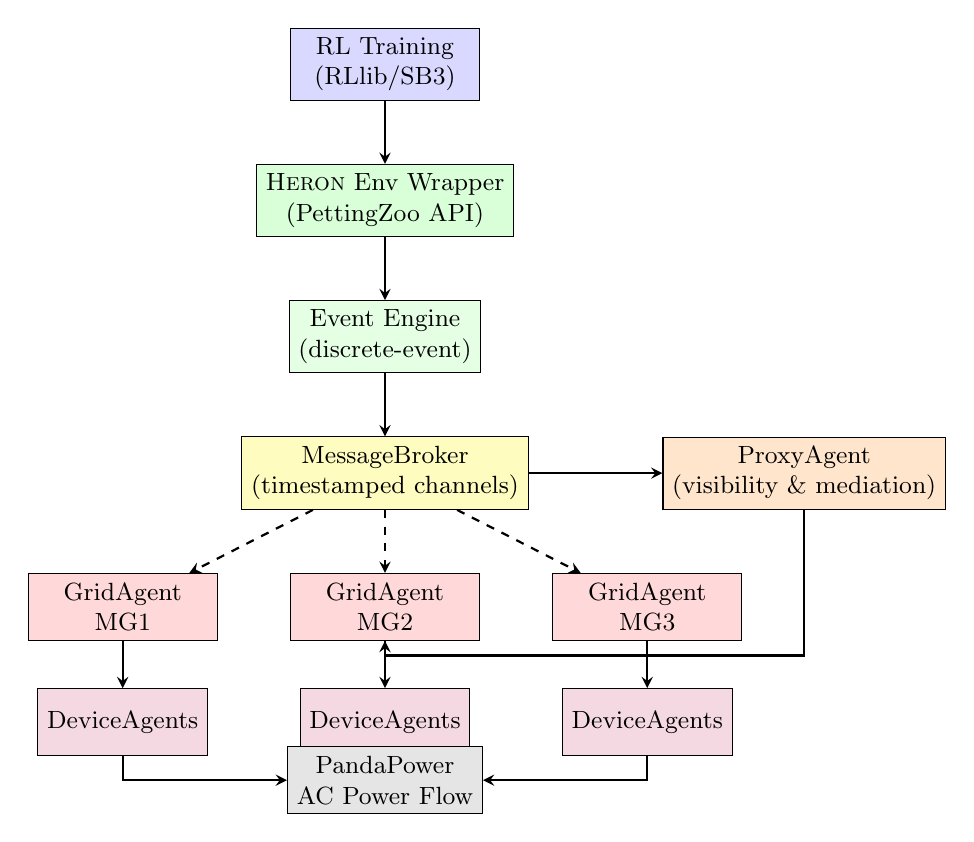
\begin{tikzpicture}[
    node distance=0.8cm,
    box/.style={rectangle, draw, minimum width=2.4cm, minimum height=0.85cm, align=center, font=\small},
    arrow/.style={->, >=stealth, thick},
    dasharrow/.style={->, >=stealth, thick, dashed}
]
% RL Layer
\node[box, fill=blue!15] (rl) {RL Training\\(RLlib/SB3)};

% Environment Layer
\node[box, fill=green!15, below=of rl] (env) {\heron{} Env Wrapper\\(PettingZoo API)};

% Event engine
\node[box, fill=green!10, below=of env] (engine) {Event Engine\\(discrete-event)};

% Message Broker
\node[box, fill=yellow!25, below=of engine] (broker) {MessageBroker\\(timestamped channels)};

% Proxy Agent
\node[box, fill=orange!20, right=1.7cm of broker] (proxy) {ProxyAgent\\(visibility \& mediation)};

% Grid Agents
\node[box, fill=red!15, below left=0.8cm and 0.3cm of broker] (ga1) {GridAgent\\MG1};
\node[box, fill=red!15, below=0.8cm of broker] (ga2) {GridAgent\\MG2};
\node[box, fill=red!15, below right=0.8cm and 0.3cm of broker] (ga3) {GridAgent\\MG3};

% Device Agents
\node[box, fill=purple!15, below=0.6cm of ga1, minimum width=1.9cm] (d1) {DeviceAgents};
\node[box, fill=purple!15, below=0.6cm of ga2, minimum width=1.9cm] (d2) {DeviceAgents};
\node[box, fill=purple!15, below=0.6cm of ga3, minimum width=1.9cm] (d3) {DeviceAgents};

% Physics
\node[box, fill=gray!20, below=3.0cm of broker] (physics) {PandaPower\\AC Power Flow};

% Arrows
\draw[arrow] (rl) -- (env);
\draw[arrow] (env) -- (engine);
\draw[arrow] (engine) -- (broker);
\draw[arrow] (broker) -- (proxy);
\draw[dasharrow] (broker) -- (ga1);
\draw[dasharrow] (broker) -- (ga2);
\draw[dasharrow] (broker) -- (ga3);
\draw[arrow] (ga1) -- (d1);
\draw[arrow] (ga2) -- (d2);
\draw[arrow] (ga3) -- (d3);
\draw[arrow] (d1.south) |- (physics.west);
\draw[arrow] (d3.south) |- (physics.east);
\draw[arrow] (proxy) |- ($(proxy.south)+(0,-1.85)$) -| (ga2);

\end{tikzpicture}
\caption{\heron{} architecture (power-system instantiation). A discrete-event engine schedules agent decisions, message deliveries, and physics updates. ProxyAgent mediates access to global state via visibility filtering; MessageBroker models explicit timestamped communication channels.}
\label{fig:architecture}
\end{figure}

%------------------------------------------------------------------------------
\subsection{Physical--Logical Decoupling via ProxyAgents}
\label{sec:proxy}
%------------------------------------------------------------------------------

A recurring deployment failure in MARL occurs when policies inadvertently exploit simulator ``omniscience''---information available to the environment implementation but unavailable to an agent in deployment. \heron{} addresses this by introducing a \textbf{ProxyAgent} that acts as the only component allowed to query the global physical state $x(\tau)$.

\paragraph{Design rule.}
Agents never directly access backend state. Instead, the ProxyAgent produces agent-specific observations by filtering a set of FeatureProviders according to visibility rules (\S\ref{sec:observability}). This enforces a clean separation between (i) \emph{physical truth} maintained by the simulator and (ii) \emph{what each agent is allowed to know}.

%------------------------------------------------------------------------------
\subsection{Composable Observability with FeatureProviders}
\label{sec:observability}
%------------------------------------------------------------------------------

Observations are assembled from composable \textbf{FeatureProviders}. Each provider maps a slice of the physical state into a vector and declares a visibility scope.

\begin{table}[t]
\centering
\caption{Visibility scopes used by \heron{} (power-domain examples shown for concreteness).}
\label{tab:visibility}
\small
\begin{tabular}{@{}lp{3.3cm}p{6.6cm}@{}}
\toprule
\textbf{Scope} & \textbf{Who can access} & \textbf{Example signals} \\
\midrule
\texttt{public} & all agents & system time, frequency/alerts \\
\texttt{owner} & owning agent only & device SOC, internal costs/constraints \\
\texttt{upper\_level} & parent in hierarchy & aggregates of subordinates, boundary conditions \\
\texttt{system} & system operator only & full network state (all buses/lines/devices) \\
\bottomrule
\end{tabular}
\end{table}

This design supports \textbf{systematic observability ablations}: a benchmark can progressively restrict what is visible (\eg \texttt{full} \,$\rightarrow$\, \texttt{upper\_level} \,$\rightarrow$\, \texttt{owner}) to quantify information requirements and expose observability-induced failure modes. \heron{} ships with 16 built-in FeatureProviders for the power instantiation (Appendix~\ref{app:featureproviders}) and an interface for user-defined providers.

%------------------------------------------------------------------------------
\subsection{Hierarchical Agents and Roles}
\label{sec:hierarchy}
%------------------------------------------------------------------------------

Many CPS are naturally hierarchical: fast local controllers, mid-level coordinators, and supervisory operators. \heron{} supports a three-level pattern that recurs across domains:
\begin{itemize}[nosep]
    \item \textbf{Level 1 (DeviceAgents)}: local actuation with \texttt{owner+public} visibility.
    \item \textbf{Level 2 (GridAgents)}: coordination over a subsystem with \texttt{upper\_level+owner+public} visibility.
    \item \textbf{Level 3 (ProxyAgent)}: system-level mediator with \texttt{system} visibility for filtering and aggregation.
\end{itemize}

This hierarchy reduces the effective joint action dimensionality and matches organizational boundaries (\eg SCADA/EMS in power systems).

%------------------------------------------------------------------------------
\subsection{Message-Based Protocols}
\label{sec:protocols}
%------------------------------------------------------------------------------

\heron{} separates \emph{coordination} from \emph{physics} through a modular protocol system.

\paragraph{Key abstraction.}
A protocol is the composition of:
\begin{enumerate}[nosep]
    \item \textbf{CommunicationProtocol}: what messages are exchanged (prices, bids, setpoints, consensus values).
    \item \textbf{ActionProtocol}: how an agent turns received messages into actuation (direct dispatch vs. decentralized response).
\end{enumerate}

This makes it possible to compare, under identical observability and latency, coordination topologies such as: (i) centralized dispatch (setpoints), (ii) hierarchical coordination (parent-to-child), and (iii) peer-to-peer mechanisms (markets, consensus). The power-system benchmark includes vertical protocols (setpoints, price signals) and horizontal protocols (P2P trading, consensus).

%==============================================================================
\section{Power-System Benchmark Instantiation}
\label{sec:power}
%==============================================================================

We instantiate \heron{} for multi-microgrid coordination using PandaPower AC power flow. The goal is not to claim a final ``leaderboard'' in this submission, but to provide a concrete CPS benchmark where timing, information structure, and coordination protocols matter.

\paragraph{Provided assets.}
\begin{itemize}[nosep]
    \item \textbf{Standard networks}: IEEE 13/34/123-bus and CIGRE LV feeders (Appendix~\ref{app:networks} for specs).
    \item \textbf{Device models}: dispatchable generators, batteries, OLTC transformers, grid connections.
    \item \textbf{Reference scenarios}: diurnal load/generation traces and contingency variants.
    \item \textbf{Baselines}: droop control and centralized MPC (where applicable).
\end{itemize}

\paragraph{Benchmark questions enabled.}
The instantiation is designed to support questions that are difficult to study in global-clock benchmarks:
\begin{itemize}[nosep]
    \item \textbf{Minimum observability for coordination}: what role-based visibility is sufficient for stable operation?
    \item \textbf{Robustness to timing uncertainty}: how do policies degrade under observation/action delays and heterogeneous decision rates?
    \item \textbf{Privacy-preserving coordination}: can microgrids coordinate without revealing internal SOC/costs?
    \item \textbf{Protocol sensitivity}: which coordination protocol is more robust under the same latency and observability constraints?
\end{itemize}

%==============================================================================
\section{What \heron{} Enables in Practice}
\label{sec:demo}
%==============================================================================

This paper's focus is the simulation/benchmarking substrate rather than final performance numbers. We therefore summarize the evaluation methodology \emph{as capabilities} and provide pilot results in the appendix.

\paragraph{Observability ablation.}
Using FeatureProviders, a single benchmark can generate an information--performance curve by progressively restricting visibility scopes (Appendix~\ref{app:pilot-results}).

\paragraph{Centralized-to-distributed mismatch.}
Dual-mode execution (centralized development vs. brokered distributed validation) enables stress-testing whether a policy trained with richer observations fails when deployed with realistic filters and latency.

\paragraph{Timing robustness.}
Because delays and decision cycles are explicit in the event engine, we can inject stochastic latency and heterogeneous actuation rates without changing the task definition.

\paragraph{Protocol studies.}
The protocol interface enables controlled comparisons of coordination mechanisms (\eg setpoint vs. price) under the \emph{same} observability and timing assumptions.

%==============================================================================
\section{Cross-Domain Reuse}
\label{sec:generalization}
%==============================================================================

Although this submission provides a full power-system benchmark, the underlying abstractions are reusable across networked systems that share three properties: (i) distributed agents with heterogeneous rates, (ii) information partitioned by roles, and (iii) explicit coordination protocols. Examples include traffic networks (signals\,$\rightarrow$\,intersections\,$\rightarrow$\,city centers) and robot fleets (robots\,$\rightarrow$\,zone managers\,$\rightarrow$\,warehouse control). We view the power instantiation as a reference template for future domain instantiations.

%==============================================================================
\section{Limitations and Future Work}
\label{sec:limitations}
%==============================================================================

\textbf{Current limitations.}
\begin{itemize}[nosep]
    \item \textbf{Communication realism}: we support configurable latency but do not yet model packet loss, corruption, or adaptive bandwidth constraints.
    \item \textbf{Dynamic observability}: visibility rules are currently configuration-driven; learning or negotiating information access is future work.
    \item \textbf{Domain breadth}: this submission includes one complete CPS benchmark (power). Additional domains require domain experts to instantiate physics and FeatureProviders.
\end{itemize}

\textbf{Power-domain limitations.}
\begin{itemize}[nosep]
    \item \textbf{Balanced-network assumption}: the current PandaPower backend targets balanced operation; extending to unbalanced distribution models is future work.
    \item \textbf{Physics solver assumptions}: we assume robust convergence of power flow; numerical non-convergence handling is not yet benchmarked.
\end{itemize}

\textbf{Next steps.}
\begin{itemize}[nosep]
    \item Standardize latency profiles (SCADA-like, V2X-like) and release protocol/observability leaderboards.
    \item Extend the event engine with message loss and adversarial perturbations (false data injection, spoofing).
    \item Develop additional instantiations (traffic, robotics) to validate cross-domain reuse.
\end{itemize}

%==============================================================================
\section{Conclusion}
\label{sec:conclusion}
%==============================================================================

We presented \heron{}, a benchmark framework built around a single organizing idea: \textbf{multi-agent simulation should make time and information structure explicit}. \heron{} replaces the global-clock, environment-centric stepping assumption with an \textbf{event-driven, agent-centric} execution model, enabling benchmarks to vary heterogeneous decision rates and latency. ProxyAgents and FeatureProviders enforce strict information boundaries, and the protocol interface supports controlled studies of coordination mechanisms.

We demonstrated benchmark readiness through a power-system instantiation with standard feeders, scenarios, and baselines. \heron{} is released open-source to support reproducible research on asynchronous, information-constrained coordination in CPS.

%==============================================================================
% References
%==============================================================================

\bibliographystyle{plainnat}
\bibliography{references}

%==============================================================================
% Appendix
%==============================================================================
\newpage
\appendix

\section{Built-in FeatureProviders (Power Instantiation)}
\label{app:featureproviders}

\begin{table}[h]
\centering
\caption{Built-in FeatureProviders for the power-system benchmark (visibility scopes shown).}
\label{tab:features}
\small
\begin{tabular}{@{}llp{6.3cm}@{}}
\toprule
\textbf{FeatureProvider} & \textbf{Visibility} & \textbf{Meaning} \\
\midrule
ElectricalBasePh & owner, upper\_level & Active/reactive power (P, Q) \\
PowerLimits & owner & Min/max capacity \\
StorageBlock & owner, upper\_level & SOC, energy capacity, charge/discharge limits \\
StatusBlock & public & Device availability/on-off \\
TapChanger & owner & Transformer tap state \\
InverterFeature & owner & Reactive capability, mode \\
BusVoltages & system, upper\_level* & Voltage magnitudes (*boundary buses for \texttt{upper\_level}) \\
LineFlows & system & Branch flows/loading \% \\
NetworkMetrics & public, system & Frequency, convergence, alerts \\
CostBlock & owner & Cost terms (fuel, degradation, ramping) \\
RampRateFeature & owner & Ramp constraints \\
SOCLimitsFeature & owner & SOC safety bounds \\
PowerFactorFeature & owner, upper\_level & PF capability \\
TemperatureFeature & owner & Thermal limits \\
ForecastFeature & owner, upper\_level & Exogenous forecasts (if available) \\
ViolationFeature & owner, upper\_level, system & Constraint violations \\
\bottomrule
\end{tabular}
\end{table}

\section{Hyperparameters}
\label{app:hyperparams}

\begin{table}[h]
\centering
\caption{MAPPO training hyperparameters (pilot experiments).}
\small
\begin{tabular}{@{}ll@{}}
\toprule
\textbf{Parameter} & \textbf{Value} \\
\midrule
Learning rate & $3 \times 10^{-4}$ \\
Discount factor ($\gamma$) & 0.99 \\
GAE lambda ($\lambda$) & 0.95 \\
Clip parameter ($\epsilon$) & 0.2 \\
Entropy coefficient & 0.01 \\
Value loss coefficient & 0.5 \\
Max gradient norm & 0.5 \\
Batch size & 4096 \\
Minibatch size & 256 \\
PPO epochs & 10 \\
Number of workers & 4 \\
Network architecture & [256, 256] \\
Activation & ReLU \\
\bottomrule
\end{tabular}
\end{table}

\section{Network Specifications}
\label{app:networks}

\begin{table}[h]
\centering
\caption{Test network specifications (power instantiation).}
\small
\begin{tabular}{@{}lcccc@{}}
\toprule
\textbf{Network} & \textbf{Buses} & \textbf{Lines} & \textbf{Voltage (kV)} & \textbf{Peak Load (MW)} \\
\midrule
IEEE 13-Bus & 13 & 11 & 4.16 & 3.5 \\
IEEE 34-Bus & 34 & 33 & 24.9 & 1.77 \\
IEEE 123-Bus & 123 & 127 & 4.16 & 3.49 \\
CIGRE LV & 14 & 13 & 0.4 & 0.245 \\
\bottomrule
\end{tabular}
\end{table}

\section{Safety Metric Definitions}
\label{app:safety}

\begin{align}
V_{\text{voltage}} &= \sum_{b \in \mathcal{B}} \left[\max(0, V_b - 1.05) + \max(0, 0.95 - V_b)\right] \\
V_{\text{loading}} &= \sum_{l \in \mathcal{L}} \max(0, \text{Loading}_l - 1.0) \\
V_{\text{SOC}} &= \sum_{s \in \mathcal{S}} \left[\max(0, 0.1 - \text{SOC}_s) + \max(0, \text{SOC}_s - 0.9)\right] \\
V_{\text{PF}} &= \sum_{d \in \mathcal{D}} \max(0, 0.85 - |\text{PF}_d|)
\end{align}

Where voltage limits are 0.95--1.05 p.u., line loading limit is 100\%, SOC safe range is 10--90\%, and minimum power factor is 0.85.

\section{Pilot Results (Preliminary)}
\label{app:pilot-results}

Values in this appendix are illustrative pilot results intended to demonstrate the benchmark's measurement capabilities; final baseline sweeps will be released with the public benchmark.

\begin{table}[h]
\centering
\caption{Example observability ablation (Summer Peak, 3 microgrids).}
\label{tab:observability-ablation}
\small
\begin{tabular}{@{}lccccc@{}}
\toprule
\textbf{Observability} & \textbf{Cost (\$)} & \textbf{Degradation} & \textbf{Safety (\%)} & \textbf{Converge (ep)} \\
\midrule
Full & \exampleval{859} & Baseline & \exampleval{2.1} & \exampleval{2400} \\
System-level & \exampleval{863} & \exampleval{+0.4\%} & \exampleval{2.3} & \exampleval{2450} \\
\textbf{Upper-level} & \exampleval{\textbf{891}} & \exampleval{\textbf{+3.7\%}} & \exampleval{\textbf{2.8}} & \exampleval{\textbf{2600}} \\
Owner-only & \exampleval{1024} & \exampleval{+19\%} & \exampleval{8.7} & \exampleval{4200} \\
Public-only & \exampleval{1543} & \exampleval{+80\%} & \exampleval{24} & Fails \\
\bottomrule
\end{tabular}
\end{table}

\begin{table}[h]
\centering
\caption{Example centralized-to-distributed mismatch (observability filtering).}
\label{tab:mode-results}
\small
\begin{tabular}{@{}lccc@{}}
\toprule
\textbf{Train visibility} & \textbf{Test visibility} & \textbf{Cost (\$)} & \textbf{Degradation} \\
\midrule
Full & Full & \exampleval{859} & -- \\
Upper-level & Upper-level & \exampleval{891} & \exampleval{-- (+3.7\% vs. full)} \\
\midrule
\textbf{Full} & \textbf{Upper-level} & \exampleval{\textbf{1055}} & \exampleval{\textbf{-23\%}} \\
\bottomrule
\end{tabular}
\end{table}

\end{document}
